\section{DAC}
%
%\begin{enumerate}
%  \item Requirements
%  \subitem >= 120ks/s
%  \subitem Fast enough digital interface
%  \subsubitem package size * samplingrate
%  \subitem Handsolder SMD package
%  \subitem 5V VCC
%  \item component/model decision
%  \item I2C vs. SPI
%  \item pcb layout
%  \item Problems with the DAC
%\end{enumerate}
%
The DAC in the Circuit is used to generate an analog voltage from the signal recorded and modulated by a Raspberry Pi or microcontroller.\p
%
As described in section \ref{sec:theory:mod} the Frequency of the modulated signal goes up to \dots$Hz$.
In order to comply with the sampling theorem, the sampling frequency of the DAC should be at least \dots$\frac{ks}{s}$. In order to meet this samplingrate, the digital interface has to bee fast enough, even if up to 7 modules are connected at the same time. Additionally the DAC should work with $5V$ supply voltage and an internal reference voltage.\p
%
I2C only allows a maximum clockspeed of $3.4MHz$ (High-speed mode). A size of a $10bit$ or $12bit$ DAC sample is usually about $32bit$ ($8bit$ Adress + RW, $8bit$ config, $10 - 12bit$ Data, $4 - 6bit$ Don't care). As shown in equation \ref{eq:pcb:dac_fs} this only allows a samplingrate up to $106.25kHz$ even if only one module is connected. Because every module needs to be addressed individual this samplingrate would drop to $15.178kHz$ when using all seven modules. For this reason SPI was selected as serial interface. SPI allows a clockfrequency up to $40MHz$ and the reciever is selected by a seperate chipselect pin wich reduces the packet size of one sample to $24bit$. Because every module gets the same signal one CS pin for all DACs can be used.\p
%
%First the 12bit DAC \dots was selected. It uses a I2C interface wich allows to connect the Raspberry Pi and the Speaker with only two wires independent of the number of modules. Unfortunately the DAC only supports a clock frequency up to $400kHz$ and each sample has a packetsize of $32bit$. As shown in equation \ref{eq:pcb:fs} this only allows a samplingrate up to $12500Hz$ even if only one module is connected.
%
\begin{align}
  f_{s,1} &= \frac{3.4MHz}{32bit} = \frac{3.4 \frac{Mbit}{s}}{32bit} = 106.25kHz \label{eq:pcb:dac_fs}\\[1em]
  f_{s, 7} &= \frac{fs_1}{7} = \frac{106.25kHz}{7} = 15.178kHz
\end{align}
%
The DAC selected fo this project is the LTC2640. It comes with an SPI interface and a samplingrate up to $125\frac{ks}{s}$. Depending on the model it supports a resolution of $8$, $10$ or $12bit$. The DAC has an internal reference voltage of $2.5V$ or $4.096V$. $12bit$ resolution with $4.096V$ reference voltage would be the ideal configuration of this DAC. Because of component shortage only the DAC with $2.5V$ reference voltage was in stock. This model produces a smaller output voltage wich can be compensated by increasing the gain of the amplifier circuit described in the next section (\ref{sec:pcb:amp}).
%
\begin{figure}
  \centering
  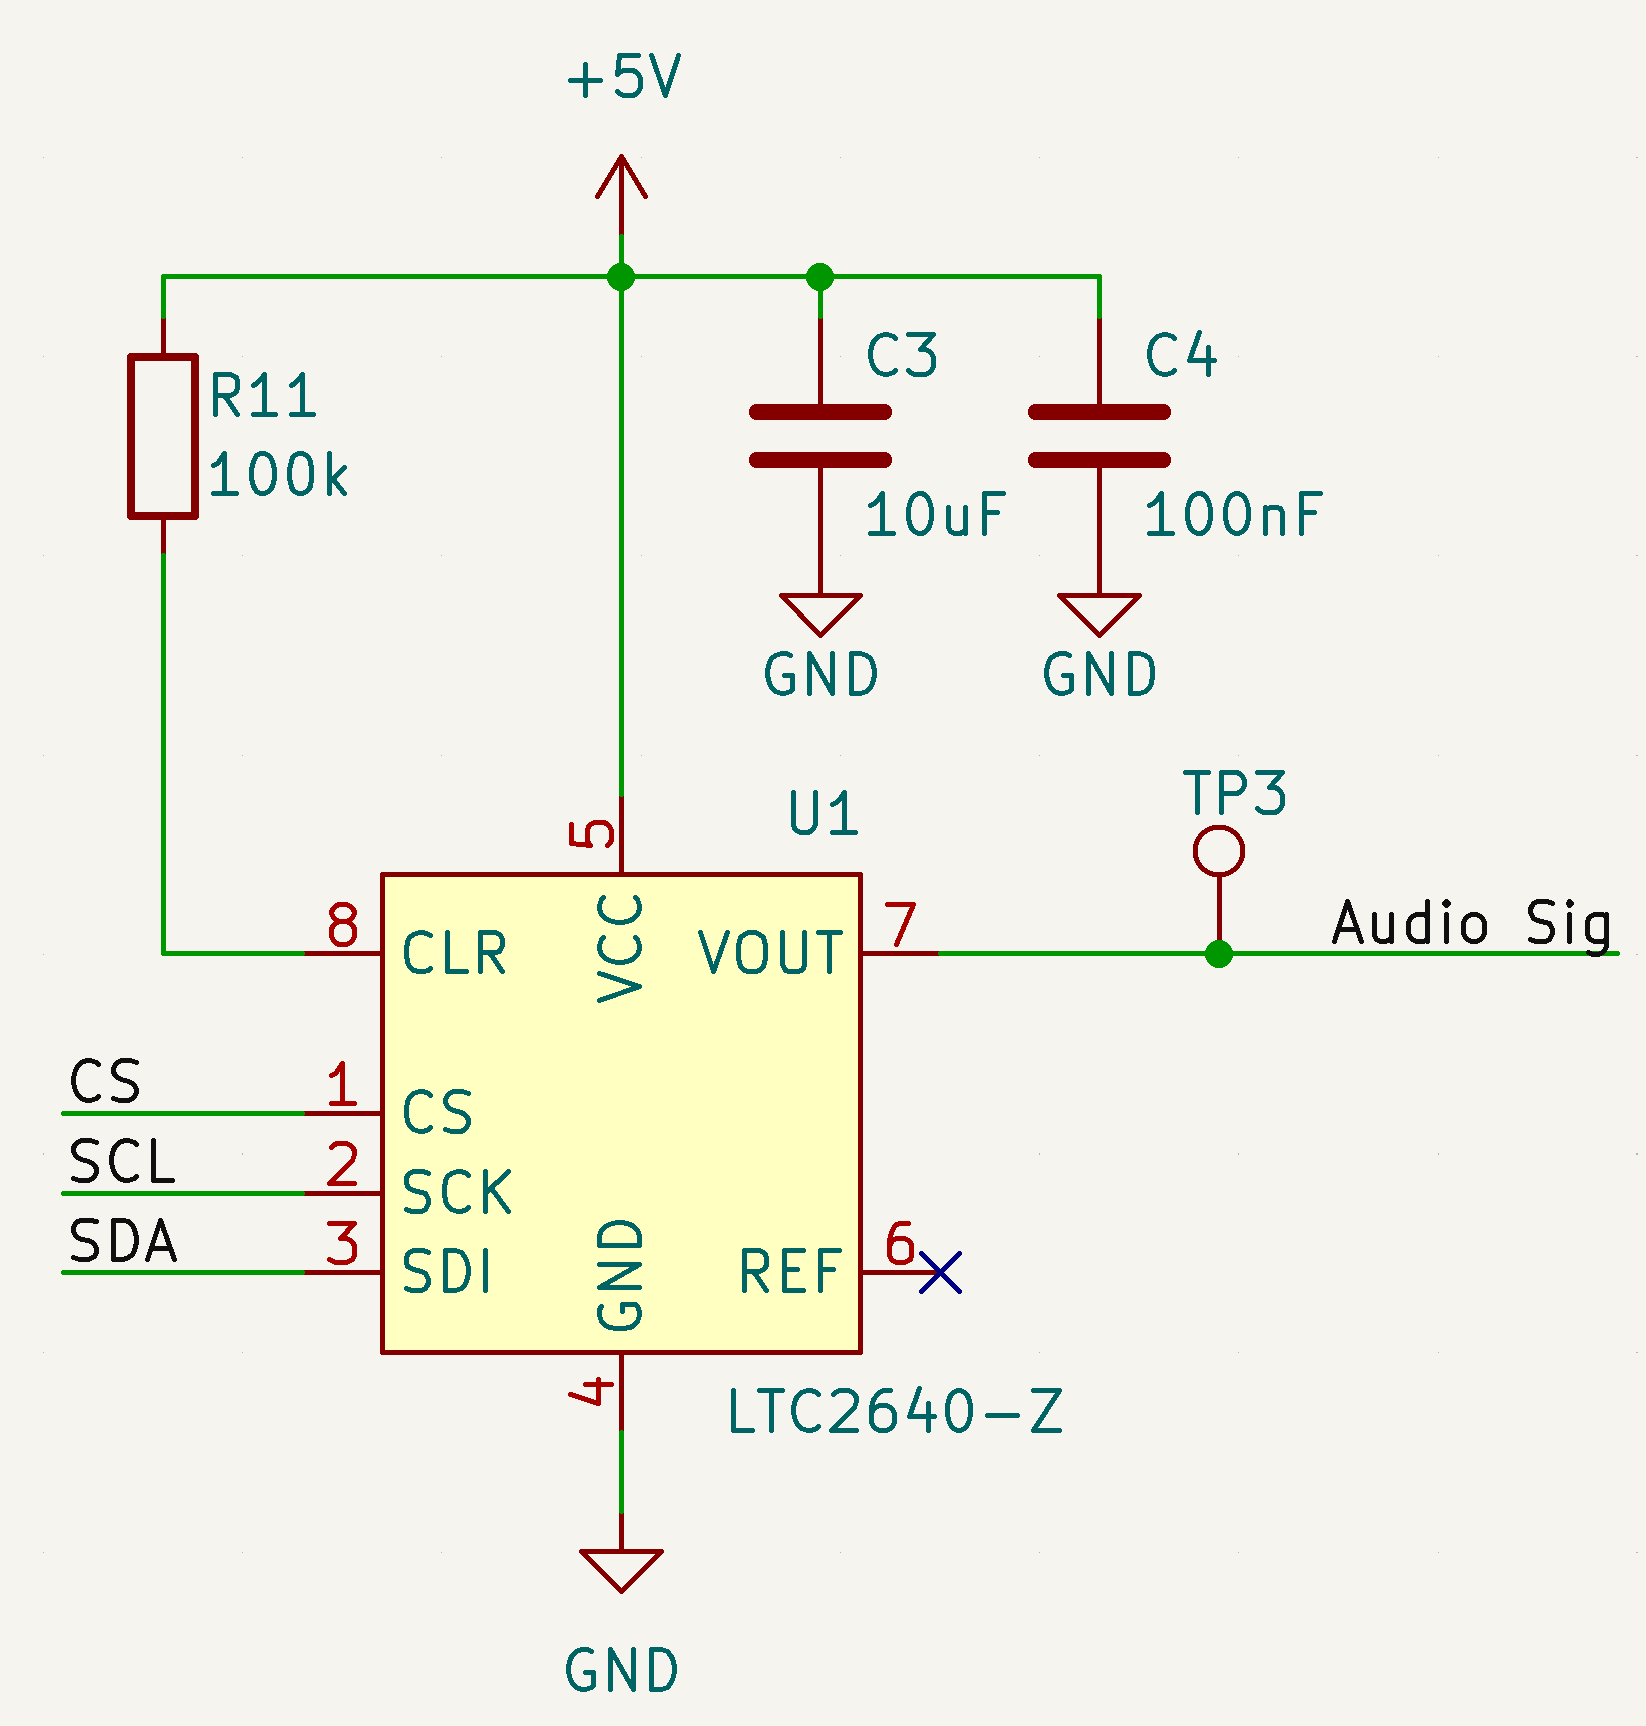
\includegraphics[height=\mediumheight]{src/assets/pictures/circuit/dac_circuit.png}
  \caption{DAC Circuit design}\label{fig:pcb:dac_circuit}
\end{figure}